%% ------------------------------------------------------------------------- %%
\chapter{Modelagem}
\label{cap:modelagem}

Utilizando-se da base de dados para modelagem descrita na seção Criação da base para modelagem (\ref{sec:criacao_da_base_para_modelagem}) - cujas variáveis explicativas foram descritas na seção Variáveis Explicativas (\ref{sec:variaveis_explicativas}) e a variável resposta descrita na seção Variável Resposta (\ref{sec:variavel_resposta}) - foram aplicados modelos de aprendizado de máquina com o intuito de obter o melhor desempenho para predição da variável resposta utilizando as variáveis explicativas construídas.

Os métodos de aprendizado de máquina utilizados foram a Regressão Linear, o Random Forest e o XGBoost, sendo que a afinação dos parâmetros de tais modelos foi feita utilizando o método Randomized Search - uma vez que é tido como mais eficiente que o Grid Search (ver (ref.)), outro método comumente utilizado. A avaliação de desempenho destes modelos foi feita utilizando-se de duas métricas, a raiz do erro quadrático médio e as bandas de acerto, e a interpretação dos modelos Random Forest e XGBoost foram feitas por meio do método Shapley Value.

\section{Análise Descritiva}
\label{sec:analise_descritiva}

A análise descritiva consiste em explorar dados utilizados para a modelagem com o intuito de encontrar a existência, ou não, de uma relação causal entre as variáveis explicativas e a variável resposta. Neste trabalho já foram apresentados algumas análises descritivas no capítulo \ref{cap:contexto}, como, por exemplo, as estatísticas dos percentuais de polaridade que representam a variável resposta.

Foram utilizadas 52 variáveis explicativas neste trabalho, assim, foi realizado uma verificação em cada uma das variáveis utilizando-se gráficos de dispersão, isto é, a exibição dos valores observados para a variável explicativa disposto em um gráfico no eixo das ordenadas e os valores observados para a variável resposta disposto no mesmo gráfico no eixo das abscissas. Como exemplo, abaixo está o gráfico de dispersão da variável 'enem_var_01_enem_score_median_pct' (cujo conceito é a mediana da nota final do enem em 2000 dividido pela mesma informação em 2010).

\graphicspath{ {./figuras/two_by_two_scatter_plot/} }
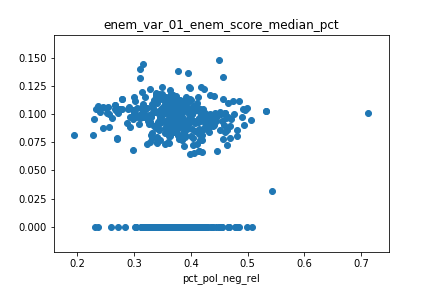
\includegraphics{28_enem_var_01_enem_score_median_pct}

O código citado no parágrafo anterior foi escrito na linguagem de programação Python utilizando a ferramenta Notebook Jupyter e se encontra no anexo \ref{ape:model_visualization}.

\section{Randomized Search}
\label{sec:randomized_search}

(?).

\section{Shapley Value}
\label{sec:shapley_value}

(?).

\section{Regressão Linear}
\label{sec:regressao_linear}

(?).

\section{Random Forest}
\label{sec:random_forest}

(?).

\section{XGBoost}
\label{sec:xgboost}

(?).

%% ------------------------------------------------------------------------- %%